%
% einleitung.tex -- Beispiel-File für die Einleitung
%
% (c) 2020 Prof Dr Andreas Müller, Hochschule Rapperswil
%
% !TEX root = ../../buch.tex
% !TEX encoding = UTF-8
%
\subsection{Zylinder\label{geodaeten:section:Linienelemente:Zylinder}}
\rhead{Linienelemente Beispiele}

Eine Kurve auf der Oberfläche eines Zylinders kann als zweidimensional betrachtet werden, wobei gilt

\begin{equation}
	\Delta s \approx \sqrt{(r \cdot \Delta \phi)^2 + \Delta z^2}
\end{equation}
und $r$ ist konstant.
Analog zu den kartesischen Koordinaten können die Abstände infinitesimal werden und das Linienelement ergibt sich dadurch für die Oberfläche des Zylinders zu

\begin{equation}
	ds^2 = \left(r^2 \cdot \dot{\phi}^2 +\dot{z}^2\right) %\cdot dt^2 .
	\label{geodaeten:equation:Linienelemente:Zylinder:equation2}
\end{equation}

%Als Vektor dargestellt entspricht das Linienelement
%
%\begin{equation}
%	\mathbf{d\vec{s}}^2 = \begin{pmatrix} r^2 \cdot \dot{\phi}^2 \\ \dot{z}^2 \end{pmatrix} = \begin{pmatrix} r^2 \\ 1 \end{pmatrix} \cdot \begin{pmatrix} \dot{\phi}^2 \\ \dot{z}^2 \end{pmatrix} \cdot dt^2 .
%\end{equation}

Den einstieg in dreidimensionale Kurven können wir machen, indem $r$ nicht als Konstant angenommen wird.
Der Weg kann so mit
\begin{equation}
	\Delta s \approx \sqrt{\Delta r^2 + (r \cdot \Delta \phi)^2 + \Delta z^2} %\cdot dt^2
\end{equation}
berechnet werden und das Linienelement entspricht 
\begin{equation}
	ds^2 = \left( \dot{r}^2 + r^2 \cdot \dot{\phi}^2 +\dot{z}^2 \right) %\cdot dt^2 .
	\label{geodaeten:equation:Linienelemente:Zylinder:Zylinder3D}
\end{equation}

%und als Vektor
%\begin{equation}
%	\mathbf{d\vec{s}}^2 = \begin{pmatrix} \dot{r}^2 \\ r^2 \cdot \dot{x}^2 \\ \dot{y}^2 \end{pmatrix} = \begin{pmatrix} 1 \\ r^2 \\ 1 \end{pmatrix} \cdot \begin{pmatrix} \dot{r}^2 \\ \dot{\phi}^2 \\ \dot{z}^2 \end{pmatrix} \cdot dt^2 .
%\end{equation}


\begin{figure}
	\centering
	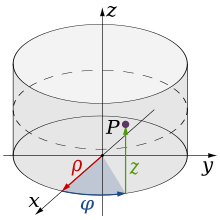
\includegraphics[width=6cm]{papers/geodaeten/Abbildungen/Linienelemente/LinZyl1}
	\caption{Linienelement im Kartesischen Raum}
	\label{geodaeten:figure:Linienelemente:Zylinder:figure2}
	\cite{geodaeten:polarkoordinaten}
\end{figure}

